\documentclass[letterpaper,12pt]{article}


\listfiles

%\usepackage{setspace}
%\doublespacing
\usepackage{pdfcomment}
%usepackage{hyperref}
\hypersetup{hidelinks}

%%  Accepte les caractères accentués dans le document (UTF-8).
\usepackage[utf8]{inputenc}
%\usepackage[french]{babel}
\usepackage[T1]{fontenc}

\usepackage[bb=boondox]{mathalfa}




%change les references aux equations
%\let\oldref\ref
%\renewcommand{\ref}[1]{\in@{eq:}{#1} \ifin@ (\oldref{#1}) \else \oldref{#1} \fi}

%commentaires
\usepackage{verbatim}

%double espacement
\usepackage{setspace}
% \doublespacing

%notes sur le pdf


%------------------------------
%packages pour tableaux
\usepackage[table,xcdraw]{xcolor}
\usepackage{rotating}

%-----------------------------

%packages pour figures
%\usepackage{fancybox}
\usepackage{epsfig}
\usepackage{graphicx}


%------------------------------------------------
%Bibliographie

%ancienne
%\usepackage[round]{natbib}
%\usepackage{numcompress}
%\bibliographystyle{model4-names}

% Natbib setup for author-year style
\usepackage{natbib}
\bibpunct[, ]{(}{)}{,}{a}{}{,}%
\def\bibfont{\small}%
\def\bibsep{\smallskipamount}%
\def\bibhang{24pt}%
\def\newblock{\ }%
\def\BIBand{and}%
\bibliographystyle{informs2014trsc}

%\usepackage[strings]{underscore}
%\bibliographystyle{plainnat}
%------------------------------------------------

%-----------------------------------------
%TIKZ
\usepackage{tikz}
\usetikzlibrary{arrows,shapes,positioning,shadows,trees}
\usetikzlibrary{patterns}
\usetikzlibrary{calc, graphs}


\tikzset{hide on/.code={\only<#1>{\color{fg!20}}}}
\tikzset{
	invisible/.style={opacity=0},
	visible on/.style={alt=#1{}{invisible}},
	alt/.code args={<#1>#2#3}{%
		\alt<#1>{\pgfkeysalso{#2}}{\pgfkeysalso{#3}} % \pgfkeysalso doesn't change the path
	},
} 
\tikzset{
	depnode/.style={circle, minimum size=0.3cm, draw, thin},
	arrnode/.style={circle, minimum size=0.3cm, draw, thin, fill=black},
	waitnode/.style={circle, minimum size=0.3cm, draw, thin, pattern = north east lines},
	sourcesinknode/.style={circle, draw, minimum size=0.3cm, line width=0.1cm},
	wait/.style={->, >=triangle 45, thin},
	nullarc/.style={->, >=open triangle 45, thin},
	flight/.style={->, >=stealth, thin},
	deadhead/.style={->, >=stealth, thin, bend left=10, dashed},
	connect/.style={->, >=open diamond, thin},
	rest/.style={->, >=diamond, thin},
	begend/.style={->, >=stealth, thick, dotted}
}
%-------------------------------------------


%packages de math
\usepackage{amssymb}
\usepackage{amsmath}

\usepackage{caption}

%packages divers
\usepackage{enumerate}
\usepackage[top=1in, bottom=1in, left=1in, right=1in]{geometry}

%packagespour tableaux
\usepackage{multirow}
%\renewcommand{\arraystretch}{0.6}

%packages et commande pour décrire les algorithmes
%\usepackage{algorithm}
%\usepackage{algorithmicx}
%\usepackage{algpseudocode}

%packages pour bibliographie

%% Vancouver numbered
%\usepackage{numcompress}\bibliographystyle{model3-num-names}
%\usepackage{natbib}
%\usepackage{bibentry}

%couleur
\usepackage{color}



%commandes personnalisées

%mettre parentheses automatiquement aux references
\let\oldref\ref
\makeatletter
\newcommand\myref[1]{\oldref{#1}}
\makeatother
%les accolades supplémentaires sont pour que tout soit inclus dans les commandes comme les exposants (on peut faire $x^\ref{...}$)
\renewcommand{\ref}[1]{{\myref{#1}}}
\renewcommand{\eqref}[1]{{(\myref{#1})}}


\newcommand{\red}[1]{{\color{red}[#1]}}
\newcommand{\new}[1]{{\bfseries#1}}
\usepackage[breakable]{tcolorbox}
\newcommand{\nouveau}[2][]{
	\begin{center}
		\begin{tcolorbox}[left=0pt, right=0pt, boxsep=5pt, width=1.03\textwidth, colframe=red!75!black,title={\textbf{\Large Nouveau! #1}},coltitle=black, colbacktitle=white, colback=white, breakable]
			#2
			
		\end{tcolorbox} 
	\end{center}
}

\newcommand{\note}[1]{\red{#1}}



%\renewcommand{\baselinestretch}{1.5} 

\title{ Optimizing the production in an open pit mine}
\author{\textsc{\large{Frédéric Quesnel}} \\ MTH6601}

%\date{\today}

%\baselineskip=15pt

\begin{document}
	
	\maketitle
	
	\setcounter{section}{-1}
	\section{Before starting...}
	
	This assignment concerns the optimization of the operations in an open-pit mine. It is based on a real research project conducted by a professor from Polytechnique. In this assignment, you will study a simplified open pit mine model using a simulator. Slides describing the mine and how the simulator works can be found on Moodle. It is strongly recommended that you review this document before you begin. For any questions concerning the simulator or this assignment, or to report a bug in the simulator, please contact Frédéric Quesnel.
	
	
	You are encouraged to include relevant tables and figures in your answers. However, you will be evaluated mainly on the quality of your analysis and your conclusions.
	
	
	%---------------------------------------------------------------------------------------------------------
	\section{Predicting travel times}
	
	The travel time of a truck over a path varies stochastically and can be influenced by various factors such as road conditions or weather. It is important to be able to correctly estimate these travel times in order to properly plan operations. In this section, you will explore three formulas that can be used to estimate travel times.
	
	
	When a truck starts a trip, a prediction formula estimates its travel time. This time is called the \textit{predicted travel time}. When the truck arrives at its destination, its \textit{observed travel time} is recorded. In the simulator, the graph entitled \textit{Temps de parcours observés et prédits} (predicted and observed travel times) displays the observed and predicted times of the trucks on two specific roads (the caption indicates which ones).
	
	Let $t_{ij}^k$ and $t^{*k}_{ij}$ be the predicted and observed times for path $(i, j)$ at moment $k$. $t_{ij}^{k-1}$ and $t^{*k-1}_{ij}$ are the predicted and observed times for the last truck that took path $(i, j)$ before $k$. Let $A$ be the set of paths. The simulation software offers the following three formulas to estimate the travel time of a truck on path $(i, j)$ : 
	
	
	
	\begin{itemize}
		
		\item \textit{Moyenne des observations précédentes }(average of the previous observed times on the same path)
		
		\begin{equation}
		t_{ij}^k = \frac{1}{n} \sum\limits_{k=1}^n t_{ij}^{*k-1}
		\end{equation}
		
		\item \textit{Combinaison convexe }(convex combination)
		
		\begin{equation}
		t_{ij}^k = \lambda t^{*k-1}_{ij} + (1-\lambda) t_{ij}^{k-1} \qquad \lambda \in [0, 1]
		\end{equation}
		
		\item \textit{Erreur précédente} (previous error)
		
		\begin{equation}
		t_{ij}^k = \lambda t^{*k-1}_{ij} + (1-\lambda) t_{ij}^{k-1} \left( 1- \frac{\sum\limits_{(l,m) \in A} t_{lm}^{k-1} - t_{lm}^{*k-1}}{\sum\limits_{(l,m) \in A} t_{lm}^{*k-1}}\right)
		\end{equation}
		
		
	\end{itemize}
	
	You can change the values of $n$ and $\lambda$ in the interface.

	
	\subsection*{Experimental protocol for this section}
	
	\begin{itemize}
		\item Mine : \textit{4 pelles}
		\item Number of trucks \textit{(Nombre de camions)} : 20
		\item Simulation time \textit{(Temps de simulation)} : 24h
		\item Scoring function \textit{(Fonction de score)} : « aléatoire » (random, default option)
	\end{itemize}
	
	Steps : 
	\begin{enumerate}
		\item Launch the simulation using the play button (to see the animation).
		\item Wait at least 3 hours of simulation (for the prediction formulas to stabilize).
		\item Vary the weather (from snowflake to sun, or vice versa).
		\item Wait for the prediction formula to stabilize again, or the end of the simulation.
	\end{enumerate}
	
	
	
	\subsection*{Question 1.1}
	
	The three functions above adapt their predictions based on previous observations. Give two desirable behaviors a prediction formula.
	
	\begin{comment}
	\textbf{Réponse : }
	
	\begin{itemize}
		\item Bonne valeur de prédiction en régime stable.
		\item S'adapte rapidement aux changements de conditions.
		\item Peu sensible aux données aberrantes (ex. si un camion tombe en panne).
	\end{itemize} 
	\end{comment}
	%L’objectif est de trouver une formule de prédiction qui réagit rapidement lors de changements drastiques des conditions de conduites sur l’ensemble de la mine.
	
	
	
	
	
	
	\subsection*{Question 1.2}
	
	Observe the behavior of the formula "average of the previous observed times on the same path" with different values of $n$. What are the advantages and disadvantages of using a greater value of $ n $.
	
	
	\subsection*{Question 1.3}
	
	We observe that the "convex combination" formula adapts faster to weather changes with greater values of $\lambda$. Should we conclude that it is better to use $ \lambda = $ 1? Why?
	
	
	\subsection*{Question 1.4}
	
	The "previous error" formula is the one that adapts the fastest to weather changes. 
	
	\begin{itemize}
		\item How do you explain this? 
		\item If other factors impacted travel times (for instance, a sudden deterioration of a road), would the formula remain valid? Justify your answer.
	\end{itemize}

	\subsection*{Question 1.5}
	In general, all prediction formulas appear more accurate on the \textit{concentrateur:pelle1} path than on the \textit{sterile:pelle3} path. How do you explain that?
	
	\subsection*{Question 1.6}
	
	For this question, assume that the transport and fill times are deterministic. Suppose $n$ trucks are on their way to an excavator ("pelle" in French) and $m$ trucks are already waiting at the excavator. Let $t_i$ be the time it takes for truck $i$ to arrive at the excavator, in seconds, and suppose that the trucks are ordered in increasing order of arrival time at the excavator ($ t_1 \leq t_2 \leq ... \leq t_{n-1} \leq t_n $). A truck is currently being filled, and that filling will be completed in $ t^r $ seconds. The filling time of a truck is $ T^R $ seconds. This situation is illustrated in figure \ref{fig:file}.
	
	\begin{figure}
		\center
		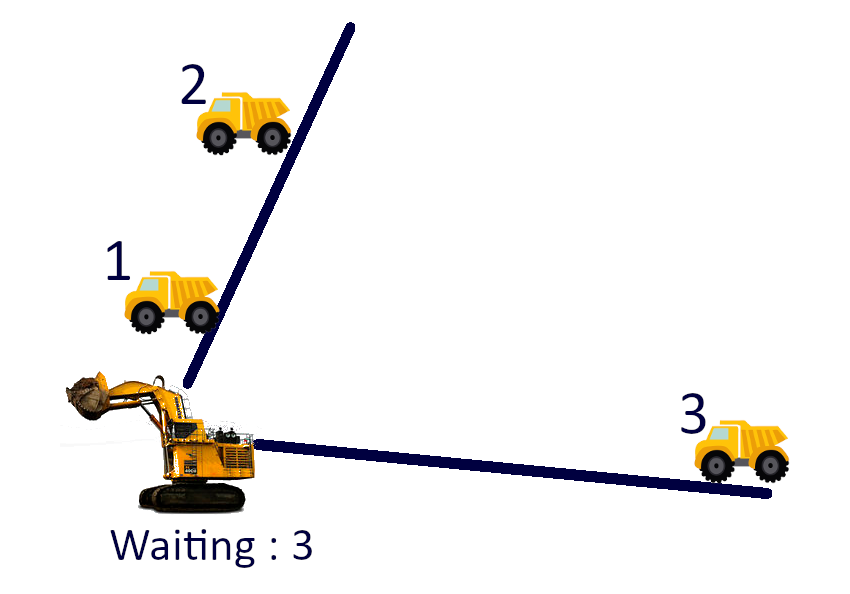
\includegraphics[width=0.4\linewidth]{File_en.png}
		\caption{\label{fig:file} }
	\end{figure}
	
	\noindent Give a formula that calculates in how long the filling of truck $n$ will start.
	
	
	\noindent \textbf{Tip :} You can use a recurrence relation.
	
	%---------------------------------------------------------------------------------------------------------
	\section{Affectation of trucks one by one}
	\label{sec:score}
	When a truck arrives at the concentrator or the waste pile (\textit{stérile} in French), it unloads instantly and becomes available. We must then assign it to a new destination. The goal of this section is to develop a rule that assigns each available truck it's next destination (excavator). This assignation is done as follows: a score is calculated for the assignment of the truck to each excavator. The excavator with the \textbf{lowest} score is chosen (in case of a tie, the excavator with the lowest number is chosen).
	

	
	\subsection*{Experimental protocol : }
	
	\begin{itemize}
		\item Mine : 10 pelles
		\item Number of trucks : 20
		\item Simulation time : 24h
		\item Scoring function : your own scoring function.
	\end{itemize}
	
	Steps : 
	\begin{enumerate}
		\item Launch the simulation using either the \textit{play} or \textit{compléter auto} button (the latter button will run the simulation faster, without animation).
		\item Save the results.
	\end{enumerate}
	
	\textbf{Tip : } Use the mine \textit{4 pelles}, or fewer trucks, to debug your scoring functions!
	
	\subsection*{Question 2.1} 
	
	You want to optimize total production (ore + waste rock), without taking into account the work plan of the excavators.

	By default, the assignment is made from the function written in the \textit{fonction de score} field of the graphical interface. You must design a scoring function using the variables provided in Section \ref{sec:vars}, as well as the basic operations (+, -, *, /, \%). Exponents can also be used using the Java function \verb|Math.pow ([base], [exopsant])|. For example, entering the formula "n1" always sends an available truck to the excavator with the fewest trucks waiting.
	
	
	Explain your scoring function choice. Do you see an increase in productivity (compared to a random assignment)? If so, by how much?

	\subsection*{Question 2.2}
	
	
	We now want to optimize production while respecting the following constraints:
	
	\begin{itemize}
		\item \textbf{Maximize : }  Ore production (to the concentrator) + 0.2 $\times$ waste rock production
		\item At most 25\% of overall production must be waste rock.
		\item Ore at the concentrator must contain at most 1.9\% of sulfur (\textit{soufre}), and between 26\% and 27\% of iron (\textit{fer}).
	\end{itemize}
	
	You must design a scoring function to achieve this goal by modifying the functions (\verb|computeDecisionScore| and \verb|computeCustomDecisionScore|) in the \verb|CustomDecisionMaker.java| file. The \verb!ComputeCustomDecisionScore! function gives you access to all trucks, excavators, and the mine in general (documentation for these classes is provided with the code). You can also use the variables defined at the beginning of the file.
	
	
	\begin{itemize}
		\item Briefly describe your function and explain the reasoning behind it.
		\item Measure the performance (averaged over several simulations) of your function (total quantity produced, compliance with production constraints, etc.)
	\end{itemize}
	
	
	
	%---------------------------------------------------------------------------------------------------------
	\section{Assignment problem}
	
	We now want to assign the trucks taking into account the trucks that will soon be available. To do this, we solve an assignment problem, as described in the presentation slides on Moodle. You can activate this option by writing "optimise" (with an s!) in the scoring function field. You can also assign the trucks one by one with the same scoring function as for the assignment problem, by writing "optimal\_assign" in the scoring function field.
	
	We also wish to take into account the \textit{plan of operations} of the mine. A plan of operations indicates the target number of trucks per hour that must go to each excavator in order to meet production needs. The target for each excavator is indicated in green next to it.
	
	\subsection*{Experimental protocol : }
	
	\begin{itemize}
		\item Mine : 10 pelles
		\item Number of trucks : 20
		\item Simulation time : 24h
		\item Scoring function : optimise.
	\end{itemize}
	
	
	
	\subsection*{Question 3.1}
	
	Give a hypothetical example where it is advantageous to use an assignment problem versus assigning trucks one by one.
	
	\subsubsection*{Question 3.2} 
	
	Perform simulations to compare the assignment of trucks "one by one" to the assignment of trucks with an assignment problem. Also compare with your results from question 2.2.
	
	What are the effects on: 

	\begin{itemize}
		\item total production.
		\item compliance with the plan.
		\item the ore composition.
	\end{itemize}
	
	\subsubsection*{Question 3.3}
	
	Using formula $c_{ij} = \left(E(AC)-AC\right)^2 + \left(E(AP)-AP\right)^2$ (see the slides on Moodle) directly in the assignment problem can sometimes be a problem. Explain why, and suggest a solution to this problem.

	
	
	
	%---------------------------------------------------------------------------------------------------------
	\section{Modifying the plan of operations}
	
	The plan of operations can be modified to meet various production goals. To modify the target of an excavator, right-click on it, click on "Modifier le plan", and enter the desired value. The maximum capacity of an excavator is \emph{6 trucks} per hour. To reset the default values, load the mine again.

	
	
	
	\subsection*{Experimental protocol : }
	
	\begin{itemize}
		\item Mine : 10 pelles
		\item Number of trucks : 20
		\item Simulation time : 24h
		\item Scoring function : optimise or optimal\_assign.
	\end{itemize}
	
	\subsection*{Question 4.1}
	Suppose the current plan is followed to the letter. Estimate what should be, over a 24-hour period :
	
	\begin{itemize}
		\item The amount of ore delivered to the concentrator.
		\item The amount of waste rock delivered to the waste pile.
		\item The percentage of iron and sulfur in the ore delivered to the concentrator.
	\end{itemize}
	
	Compare those numbers with the results of a simulation.

	
	\subsection*{Question 4.2}
	Assuming that any plan can be followed to the letter, write a linear optimization model that determines the best plan of continuous operations.
	
	\begin{itemize}
		\item \textbf{Maximize : } Ore production (to the concentrator) + 0.2 $\times$ waste rock production
		\item At most 25\% of overall production must be waste rock.
		\item Ore at the concentrator must contain at most 1.9\% of sulfur (\textit{soufre}), and between 26\% and 27\% of iron (\textit{fer}).
	\end{itemize}
	
	Using an optimization software (the Excel linear solver, for instance), solve this problem and give its solution. Answer the first part of question 4.1 using that plan (without performing any simulation).

	
	\subsection*{Question 4.3}
	
	Simulate the plan found in 4.2. Compare the simulation results with the predictions of the optimization software. What do you think explains these differences? In other words, what are the elements that the linear optimization model does not consider?

	
	\subsection*{Question 4.4}
	
	Propose a plan of operations that allows all constraints to be respected in a simulation. Simulate this plan and give its production characteristics.
	
	\subsection*{Question 4.5}
	Linear models tend to produce extreme solutions. Explain how this could be a problem with the model developed in 4.2.
	
	
	
	
	
	
	\section{Optimizing production costs}
	%---------------------------------------------------------------------------------------------------------
	
	If the cost for a minute of waiting for an excavator is $ 10, and waiting for a truck costs $ 3 / minute, estimate the optimal number of trucks (number of trucks that minimizes the total cost of waiting)? Use the default plan.
	
	
	\section*{Bonus question}
	It might be useful to develop a tool that tells the planner if her plan is realistic.
	
	Write an optimization problem that calculates the smallest number of trucks needed to perform a given plan. (Hint: this is a transport problem that minimizes the \underline{total} truck operating time in continuous mode).
	
	
	\section{Liste of variables}
	\label{sec:vars}
	
	
	\begin{itemize}
		\setlength\itemsep{0.01em}
		\item $x1$ : Average speed of a truck.
		\item $x2$ : 1 if the excavator is currently working, 0 otherwise.
		\item $x3$ : Random real (well, rational...) number between 0 et 1.
		\item $x4$ : Infinity (which is $(2-2^{-52})*2^{1023}$ for doubles in Java)
		\item $t1$ : Average fill time of a truck.
		\item $t2$ : Expected value of the travel time to the excavator.
		\item $d1$ : Distance between the truck and the excavator.
		\item $n1$ : Number of trucks waiting at the excavator (not counting the truck being filled).
		\item $n2$ : Number of trucks at the excavator (counting the one being filled).
		\item $n3$ : Number of trucks on their way to the excavator.
		\item $t3$ : Expected time for the excavator to fill all trucks currently waiting.
		\item $t4$ : Expected time before the excavator begins to fill the truck.
		\item $t5$ : Expected waiting time of the truck (0 if the excavator is inactive when the truck arrives).
		\item $t6$ : Expected waiting time of the excavator (can be negative if the excavator is busy when the truck arrives).
	\end{itemize}
	
	
	
\end{document}

